% Roll Number 15, Aparna V K
\textbf{\textcolor{LightMagenta}{Describe any two techniques used for Ensemble learning. (December 2019 - Q7) \hfill 4 marks}} \\[5pt]


Ensemble methods are techniques that create multiple models and then combine them to produce improved results. Ensemble methods usually produces more accurate solutions than a single model would. 
\\ \textbf{Bagging} and \textbf{Stacking} are two of the ensemble methods. 
\textcolor{purple}{\subsubsection*{Bagging- \textbf{B}ootstrap \textbf{Agg}regating}}
The idea behind bagging is combining the results of multiple models (for instance, all decision trees) to get a generalized result.

\textcolor{purple}{\underline{\smash{Bootstrapping}}} is a sampling technique in which we create subsets of observations from the original dataset, with replacement. The size of the subsets is the same as the size of the original set.

\textcolor{purple}{\underline{\smash{Bagging(or Bootstrap Aggregating)}}}  technique uses these subsets (bags) to get a fair idea of the distribution (complete set). The size of subsets created for bagging may be less than the original set.
\begin{enumerate}
    \item Multiple subsets are created from the original dataset, selecting observations with replacement.
    \item A base model (weak model) is created on each of these subsets.
    \item The models run in parallel and are independent of each other.
    \item The final predictions are determined by combining the predictions from all the models.
\end{enumerate}
\begin{center}
    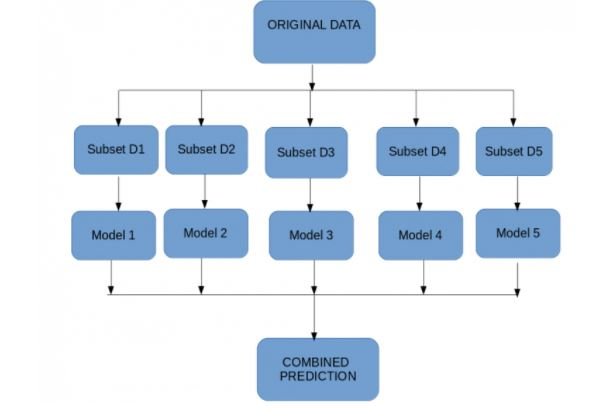
\includegraphics[width=10cm]{Images/A8_img1.jpg}
\end{center}
\subsubsection*{\textcolor{purple}{Stacking}}
Stacking is an ensemble learning technique that uses predictions from multiple models (for example decision tree, knn or svm) to build a new model. This model is used for making predictions on the test set. Below is a step-wise explanation for a simple stacked ensemble:
\begin{enumerate}
    \item The train set is split into 10 parts.
    \item A base model (suppose a decision tree) is fitted on 9 parts and predictions are made for the 10th part. This is done for each part of the train set.
    \item The base model (in this case, decision tree) is then fitted on the whole train dataset.
    \item Using this model, predictions are made on the test set.
    \item Steps 2 to 4 are repeated for another base model (say knn) resulting in another set of predictions for the train set and test set.

    \item The predictions from the train set are used as features to build a new model.
    \item This model is used to make final predictions on the test prediction set.
\end{enumerate}
\begin{center}
   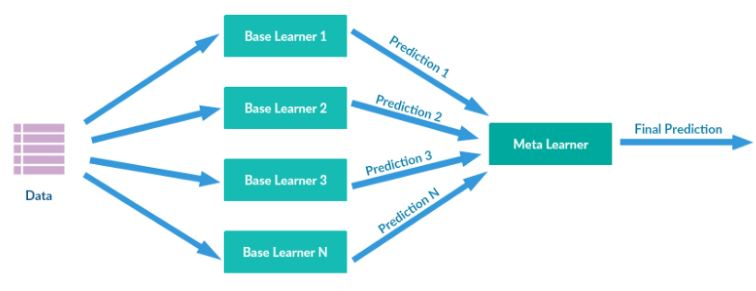
\includegraphics[height=6cm]{Images/A8_img2.jpg}
\end{center}
